\section{Preliminaries}\label{sec:prelim}
In this section we briefly recap the necessary background both from the fields of pattern mining and Answer Set Programming (ASP). 

Let $\mi{D}$ be a dataset, $\patternspace$ a language for expressing pattern properties or defining subgroups of the
data, and $\mi{q}$ a selection predicate. %Then t
The task of pattern mining is to find $\mi{Th}(\patternspace,D, \mi{q})= \{\phi \in \patternspace \mid \mi{q}(D, \phi) \text{ is true}\}$, that is, to find all patterns $\phi\in\patternspace$ that are selected by $q$  (see, e.g, the seminal work of \textcite{DBLP:journals/datamine/MannilaT97}). 

Pattern mining has been mainly studied for % in three settings: 
itemsets, sequences, graphs and tilings. These settings are determined by the language of $\patternspace$. In this work we discuss all of these pattern types.

\subsection{Patterns} 
\subsubsection{Itemsets}
 \emph{Itemsets} represent the most simple setting of frequent pattern mining. Let $\cI$
be a set of items $\{o_1,o_2,\dotsc,o_n\}$. A nonempty subset of $\cI$ is called an \emph{itemset}. A
\emph{transaction dataset} $D$ is a collection of itemsets, $D = \{t_1 ,\dotsc, t_m \}$, where $t_i\subseteq \cI$.
For any itemset $\alpha$, we denote the set of transactions that contain $\alpha$ as $D_{\alpha}= \{i\mid\alpha \subseteq t_i, t_i \in D\}$; we refer to $D_{\alpha}$ as the \emph{cover} of an itemset $\alpha$ and to $\abs{D_{\alpha}}$ as the \emph{support (frequency)} of $\alpha$ in $D$, written $\mi{sup}(\alpha)$. The \emph{relative frequency} of $\mi{\alpha}$ in $D$ refers to the ratio between $\mi{sup}(\alpha)$ and $\abs{D}$. %Moreover, we 
The \emph{cardinality} (or \emph{size}) $\abs{\alpha}$ of an itemset $\alpha$ is %defined as 
the number of items contained in it. %, i.e., $|\alpha| = |\{o_i \,|\,o_i \in \alpha\}|$.

\begin{definition}[Frequent Itemset]\label{def:frit} 
 Given a transaction dataset $D$ and a frequency threshold $\sigma \geq 0$, an itemset $\alpha$ is \emph{frequent} in $D$ if  $\mi{sup}(\alpha)\geq \sigma$.\footnote{In \emph{frequent pattern mining}, often, a \emph{relative threshold}, i.e., $\sigma/\abs{D}$ is specified by the user.}
\end{definition}

We illustrate the introduced notions by the following example.

\begin{example}\label{ex:it}
Consider a transaction dataset $D$ from Table~\ref{tab:it}.
We have %that 
$\cI=\{a,b,c,d,e\}$ and $\abs{D}=3$. For $\sigma=2$, the following itemsets are frequent: $\alpha_1{=}\{a\}$, $\alpha_2{=}\{b\}$, $\alpha_3{=}\{e\}$, $\alpha_4{=}\{a,e\}$ and $\alpha_5{=}\{b,e\}$. Moreover, it holds that $D_{\alpha_4}=\{1,3\}, D_{\alpha_5}=\{1,2\}$, and the coverage for the rest of the itemsets can be analogously found. \qed
\end{example}



\begin{table}[t]
    \begin{minipage}{.5\linewidth}
      \centering
\begin{tabular}{|l|l|l|l|l|l|}
\hline
$\mi{ID}$& $\mi{a}$ &$\mi{b}$&$\mi{c}$&$\mi{d}$&$\mi{e}$\\ \hline
$\mi{1}$ & $\checkmark$ &$\checkmark$ &&$\checkmark$&$\checkmark$\\ \hline
$\mi{2}$ &  &$\checkmark$ &$\checkmark$&&$\checkmark$\\ \hline
$\mi{3}$ &$\checkmark$ &&&&$\checkmark$ \\ \hline
\end{tabular}
      \caption{Transaction database}
\label{tab:it}
    \end{minipage}%
    \begin{minipage}{.5\linewidth}
      \centering
\begin{tabular}{|l|l|}
\hline
$\mi{ID}$& Sequence\\ \hline
$\mi{1}$ & $\tuple{\mi{a\,b\,c\,d\,a\,e\,b}}$ \\ \hline
$\mi{2}$ & $\tuple{\mi{b\,c\,e\,b}}$\\ \hline
$\mi{3}$ & $\tuple{\mi{a\,a\,e}}$ \\ \hline
\end{tabular}
      \caption{Sequence database}
\label{tab:seq}

    \end{minipage} 
\label{tab:ex}
\end{table}

\begin{figure}
    \begin{subfigure}[b]{0.3\textwidth}
        \centering
        \resizebox{\linewidth}{!}{
       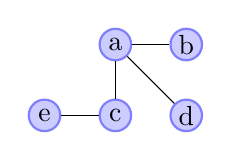
\begin{tikzpicture}[scale=0.9,
        circ/.style={circle,draw=blue!50,fill=blue!20,thick,
          inner sep=0pt,minimum size=4mm},
        transition/.style={rectangle,draw=black!50,fill=black!20,thick,
          inner sep=0pt,minimum size=4mm}]
      \node (1) at ( 0,2) [circ] {a};
      \node (2) at ( 1,2) [circ] {b};
      \node (3) at ( 0,1) [circ] {c};
      \node (4) at ( 1,1) [circ] {d};
      \node (5) at ( -1,1) [circ] {e};
      \draw (1) edge[-] (2);
      \draw (1) edge[-] (3);
      \draw (1) edge[-] (4);
      \draw (3) edge[-] (5);
\end{tikzpicture}     


        }
        \caption{Graph $G_1$}
        \label{fig:g1}
    \end{subfigure}
    \begin{subfigure}[b]{0.3\textwidth}
    \centering
        \resizebox{\linewidth}{!}{
           
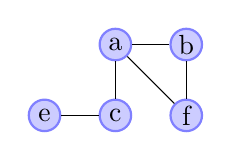
\begin{tikzpicture}[scale=0.9,
        circ/.style={circle,draw=blue!50,fill=blue!20,thick,
          inner sep=0pt,minimum size=4mm},
        transition/.style={rectangle,draw=black!50,fill=black!20,thick,
          inner sep=0pt,minimum size=4mm}]
      \node (1) at ( 0,2) [circ] {a};
      \node (2) at ( 1,2) [circ] {b};
      \node (3) at ( 0,1) [circ] {c};
      \node (4) at ( 1,1) [circ] {f};
      \node (5) at ( -1,1) [circ] {e};
      \draw (1) edge[-] (2);
      \draw (1) edge[-] (3);
      \draw (1) edge[-] (4);
      \draw (3) edge[-] (5);
      \draw (2) edge[-] (4);
\end{tikzpicture}

        }
        \caption{Graph $G_2$}   
        \label{fig:g2}
    \end{subfigure}
    \begin{subfigure}[b]{0.3\textwidth}
        \centering
        \resizebox{\linewidth}{!}{
  
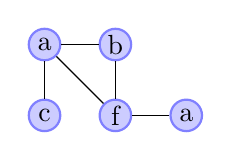
\begin{tikzpicture}[scale=0.9,
        circ/.style={circle,draw=blue!50,fill=blue!20,thick,
          inner sep=0pt,minimum size=4mm},
        transition/.style={rectangle,draw=black!50,fill=black!20,thick,
          inner sep=0pt,minimum size=4mm}]
      \node (1) at ( 0,2) [circ] {a};
      \node (2) at ( 1,2) [circ] {b};
      \node (3) at ( 0,1) [circ] {c};
      \node (4) at ( 1,1) [circ] {f};
      \node (5) at ( 2,1) [circ] {a};
      \draw (1) edge[-] (2);
      \draw (1) edge[-] (3);
      \draw (1) edge[-] (4);
      \draw (4) edge[-] (5);
      \draw (2) edge[-] (4);
\end{tikzpicture}

        }
        \caption{Graph $G_3$}
        \label{fig:g3}
    \end{subfigure}
\bigskip

\caption{Graph examples} 
\label{fig:graphs}
\end{figure}



\subsubsection{Sequences} A \emph{sequence} is an ordered set of items $\tuple{s_1,\dotsc,s_n}$.
The setting of \emph{sequence mining} includes two related yet different cases: frequent substrings 
and frequent subsequences. In this work we focus on the latter. 


\begin{definition}[Embedding in a Sequence]\label{def:embseq}
Let $S=\tuple{s_1,\dotsc,s_m}$ and $S'=\tuple{s_1',\dotsc,s_n'}$ be  two  sequences  of  size $m$ and $n$ respectively  with $m \leq n$.  The  tuple  of  integers $e=(e_1,\dotsc,e_m)$ is an \emph{embedding} of $S$ in $S'$ (denoted $S\sqsubseteq_e S')$ if and only if $e_1< \dotsc < e_m$ and for any $i \in \{1,\ldots,m\}$ it holds that $s_i=s'_{e_i}$.
\end{definition}


\begin{example}\label{ex:seq}
	For \revision{the} dataset in Table ~\ref{tab:seq} we have that $\tuple{b\,c\,e\,b} \sqsubseteq_{e_1} \tuple{\mi{a\,b\,c\,d\,a\,e\,b}}$ for $\mi{e_1}=(2,3,6,7)$ and analogously, $\tuple{\mi{a\,a\,e}}\sqsubseteq_{e_2} \tuple{\mi{a\,b\,c\,d\,a\,e\,b}}$ with $e_2=(1,5,6)$. \qed
\end{example}

We are now ready to define an inclusion relation for sequences. 

\begin{definition}[Sequence Inclusion]\label{def:seqinc}
Given two sequences $S = \tuple{s_1,\dotsc, s_m}$ and $S'=\tuple{s_1',\dotsc, s_n'}$, of %length 
size $m$ and $n$, respectively, with $m \leq n$, we say that $S$ is \emph{included} in $S'$ or $S$ is a \emph{subsequence} of $S'$ denoted by $S \sqsubseteq S'$ iff an embedding $e$ of $S$ in $S'$ exists, i.e.
\begin{equation}
S \sqsubseteq S' \leftrightarrow \exists e_1<\dotsc<e_m \text{ and }\forall i \in 1\dotsc m: s_i=s_{e_i}'.
\end{equation}
\end{definition}

\begin{example}
  In Ex.~\ref{ex:seq} we have  $\tuple{b\,c\,e\,b} \sqsubseteq \tuple{\mi{a\,b\,c\,d\,a\,e\,b}}$ but  $\tuple{\mi{a\,a\,e}} \not \sqsubseteq \tuple{\mi{b\, c\, e\, b}}$. \qed
\end{example}

For a given sequence $S$ and a sequential dataset $D=\{S_1,\dotsc,S_n\}$ we denote by $D_S$ the subset of $D$ s.t. $S \sqsubseteq S'$ for all $S' \in D_S$. The support of $S$ is $\mi{sup}(S)=\abs{D_S}$. Frequent sequences are defined analogously to frequent itemsets. 
%Let $D_S$ be the subset of $D$ such that $S\sqsubseteq S'$ for all $S' \in D_S$ for a given sequential dataset $D=\{S_1,\dotsc, S_n\}$ and a sequence $S$.

\begin{definition}[Frequent Sequence]\label{def:frseq} Given a sequential dataset $D=\{S_1,\dotsc, S_n\}$ and a frequency threshold $\sigma \geq 0$, a sequence $S$ is \emph{frequent} in $D$ if $\mi{sup}(S)\geq \sigma$. %, where $\sigma \geq 0$ is a user-specified minimum \emph{support}. 
\end{definition}

\begin{example}
	For \revision{the} dataset in Table~\ref{tab:seq} and $\sigma=2$, it holds that $\tuple{\mi{b\,c\,e\,b}}$ and $\tuple{a\,a\,e}$ are frequent, while $\tuple{\mi{b\,d\,b}}$ is not. \qed
\end{example}

Note that $\sqsubseteq$ and $\subseteq$ are incomparable relations. Indeed, consider two sequences $s_1=\tuple{a\,b}$ and $s_2=\tuple{b\,a\,a}$. While $s_1\subset s_2$, we clearly have that $s_1 \not \sqsubset s_2$.

\subsubsection{Graphs} A \emph{graph} $G$ is a triple $\tuple{V, E, l}$ where $V$ is a set of vertices, $E$ is a set of edges and $l$ is a labeling function that maps each edge and each vertex to a label. 

In this work we consider undirected graphs. Moreover, we primarily focus on two settings: a general one, where labels of the graph are not necessarily unique and a more restricted one, where unique labels are ensured.

\revision{\paragraph{General Case of Graph Mining.} Here we consider the general case of mining graphs whose nodes have labels that are not necessarily unique. This setting is computationally harder than the special case of uniquely labelled graphs. In this general setting, a pattern is an arbitrary graph with labeled nodes and edges.}
\revision{\paragraph{Uniquely Labelled Graphs.} In this restricted case, the labeling function assigns unique labels to the nodes, i.e., each node has a unique label within this graph (in the setting, no labels is assumed on the edges). This restriction makes sub-pattern check computationally easier and allows certain reductions to other pattern mining problems as indicated below.}

\begin{example}
    The graphs in Figure~\ref{fig:g1} and \ref{fig:g2} are unique-labeled ones, while the graph from Figure~\ref{fig:g3} is clearly not. \qed
\end{example}

\revision{Throughout the text we assume the general case unless stated otherwise, all experimental results have been provided for the general case of graph mining.}


\begin{definition}[Graph Isomorphism]\label{def:isom}
    Given two graphs $G=\tuple{V,E,l}$ and $G'=\tuple{V',E',l'}$, we say that $G$ is isomorphic to $G'$ iff there is a \revision{bijective function} $f$ such that 
    \revision{
        \begin{itemize}
            \item $v \in V$ iff $f(v)\in V'$ and for all $v \in V$ it holds that $l(v)=l'(f(v))$
            \item $e \in E$ iff $f(e)\in E'$ and for all $e \in E$ it holds that $l(e)=l'(f(e))$.
        \end{itemize}
    }
\end{definition}



In the general setting, the problem of deciding whether a subgraph isomorphism exists is NP-complete. However, several restricted settings have been identified, for which the problem can be solved in polynomial time, e.g., unique-labelled undirected graphs \parencite{DBLP:journals/corr/abs-1709-00900}.

\begin{definition}[Graph Inclusion]\label{def:subgraph}
    Given two graphs $G = \tuple{V,E}$ and $H=\tuple{U, F}$, such that $|V|\leq |F|$, we say that $G$ is an \emph{(isomorphic) subgraph} of $H$  denoted by $G \sqsubseteq H$ iff there exists a subgraph $H' = \tuple{U'\subseteq U, F'\subseteq F}$ such that $G$ is isomorphic to $H'$.
\end{definition}

\begin{example}
    Graph $G'_1$ of Figure~\ref{fig:subgraphs} is an isomorphic subgraph of graphs $G_1$ and $G_2$ of Figure~\ref{fig:graphs}; it is not isomorphic to graph $G_3$. Graph $G'_2$ is isomorphic to graphs $G_2$ and $G_3$, but it is not isomorphic to graph $G_1$.  \qed
\end{example}
% We say a graph G occurs in a transaction (tid, H) of a dataset D iff G is isomorphic to a subgraph of H: G v H.
% While checking the subset relation is relatively simple, especially when itemsets are implemented as bitvectors, for
% graphs this requires solving the subgraph isomorphism problem which is NP complete [Coo71]. \comment{DS: TODO add background on graphs}

\begin{figure}
    \begin{subfigure}[b]{0.3\textwidth}
        \centering
        \resizebox{\linewidth}{!}{
            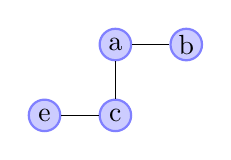
\begin{tikzpicture}[scale=0.9,
                circ/.style={circle,draw=blue!50,fill=blue!20,thick,
                inner sep=0pt,minimum size=4mm},
                transition/.style={rectangle,draw=black!50,fill=black!20,thick,
                inner sep=0pt,minimum size=4mm}]
                \node (1) at ( 0,2) [circ] {a};
                \node (2) at ( 1,2) [circ] {b};
                \node (3) at ( 0,1) [circ] {c};
                \node (5) at ( -1,1) [circ] {e};
                \draw (1) edge[-] (2);
                \draw (1) edge[-] (3);
                \draw (3) edge[-] (5);
            \end{tikzpicture}     
        }
        \caption{Graph $G'_1$}
        \label{fig:sg1}
    \end{subfigure}
    \begin{subfigure}[b]{0.3\textwidth}
        \centering
        \resizebox{\linewidth}{!}{
            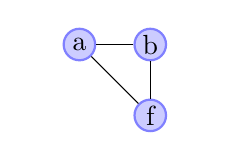
\begin{tikzpicture}[scale=0.9,
                circ/.style={circle,draw=blue!50,fill=blue!20,thick,
                inner sep=0pt,minimum size=4mm},
                transition/.style={rectangle,draw=black!50,fill=black!20,thick,
                inner sep=0pt,minimum size=4mm}]
                \node (1) at ( 0,2) [circ] {a};
                \node (2) at ( 1,2) [circ] {b};
                \node (4) at ( 1,1) [circ] {f};
                \node at (-0.6,1) {};
                \node at (1.6,1) {};
                \draw (1) edge[-] (2);
                \draw (1) edge[-] (4);
                \draw (2) edge[-] (4);
            \end{tikzpicture}  
        }
        \caption{Graph $G'_2$}
        \label{fig:sg2}
    \end{subfigure}
    \caption{Isomorphic subgraphs for graphs in Figure~\ref{fig:graphs}} 
    \label{fig:subgraphs}
\end{figure}


\subsection{Condensed pattern representations under constraints}
In data mining, constraints are typically specified by the user to encode domain background knowledge. \textcite{DBLP:conf/cpaior/NegrevergneG15} distinguish four types of constraints: 1) constraints over the pattern (e.g., restriction on its %length
size), 2) constraints over the cover set (e.g., minimal frequency), 3) constraints over the inclusion relation (e.g., maximal allowed gap in sequential patterns) and 4) constraints over the solution set (e.g., condensed representations).  

Orthogonally, constraints can be classified into \emph{local} and \emph{global} ones.  
A constraint is \emph{local} if deciding whether a given pattern satisfies it is possible without looking at other patterns. For example, minimal frequency or maximal pattern %length 
size are local constraints. On the contrary, deciding whether a pattern satisfies a \emph{global} constraint requires comparing it to other patterns. All constraints from the fourth group are global ones. We are interested in global constraints related to condensed representations. 

As argued in Sec.~\ref{sec:intro}, the order in which constraints are applied influences the solution set \parencite{DBLP:journals/kais/BonchiL06}. %In this work w
%We take the same view a
Following \textcite{DBLP:journals/kais/BonchiL06}, in this work we %and %aim at 
apply %ing 
global constraints only after local ones.

We now present the notions required in our pattern mining framework. Here, the definitions are given for itemsets; for sequences and graphs they are identical up to substitution of $\subset$ with $\sqsubset$ (subsequence relation). First, to rule out patterns that do not satisfy some of the local constraints, we introduce the notion of validity.

\begin{definition}[Valid pattern under constraints]\label{def:val}
    Let $C$ be a constraint function \revision{(local constraint)} from \patternspace to $\{ \top, \bot \}$ and let $p$ be a pattern in \patternspace. Then the pattern $p$ is called \emph{valid} iff $C(p) = \top$; otherwise it is referred \revision{to} as \emph{invalid}.
\end{definition}


\begin{example}\label{ex:valid}
    Let $C$ be a constraint function checking whether a given pattern is of size %has length 
    at least 2. Then in Ex.~\ref{ex:it}, we have $C(\alpha_i)=\bot$, $i\in\{1,2,3\}$, and $C(\alpha_j)=\top$, $j\in\{4,5\}$. \qed
\end{example}

For detecting patterns that satisfy a given global constraint, the notion of \emph{dominance} is of crucial importance. Intuitively, a dominance relation reflects pairwise preference ($\subpattern$)
between patterns and it is specific for each mining setting.  In this work we primarily focus on global constraints related to maximal, closed, free and skyline condensed representations, for which $\subpattern$ is defined as follows:

\begin{itemize}
    \item[(i)] \textbf{Maximal.} For itemsets $p$ and $q$, $p \subpattern q$ holds iff $p \subset q$
    \item[(ii)] \textbf{Closed.} For itemsets $p$ and $q$, $p \subpattern q$ holds iff $p \subset q$ and  $\mi{sup}(p) = \mi{sup}(q)$ 
    \item[(iii)] \textbf{Free.} For itemsets $p$ and $q$, $p \subpattern q$ holds iff $q \subset p$ and $\mi{sup}(p) = \mi{sup}(q)$ 
    \item[(iv)] \textbf{Skyline.} For itemsets $p$ and $q$, $p \subpattern q$ holds iff 
        \begin{itemize}
            \item[(a)] $\mi{sup}(p) \leq \mi{sup}(q)$ and $\size(p) < \size(q)$ or 
            \item[(b)] $\mi{sup}(p) < \mi{sup}(q) $ and $\size(p) \leq \size(q)$
        \end{itemize}
\end{itemize}

Dominated patterns under constraints are now formally defined.

\begin{definition}[Dominated pattern under constraints]\label{def:dom}
    Let $C$ be a constraint function, and let $p$ be a pattern, then $p$ is called \emph{dominated} iff there exists a pattern $p' \in \patternspace$ such that $p \subpattern p'$ and $p'$ is valid under $C$.
\end{definition}

\begin{example}
    In Ex.~\ref{ex:it} for the maximality constraint we have that $\alpha_1$ is dominated by $\alpha_4$, $\alpha_2$ by $\alpha_5$, while $\alpha_3$ both by $\alpha_4$ and $\alpha_5$. \qed
\end{example}

Exploiting the above definitions we obtain condensed patterns under constraints.

\begin{definition}[Condensed pattern under constraints]\label{def:con}
    Let $p$ be a pattern from \patternspace, and let $C$ be a constraint function, then a pattern $p$ is called \emph{condensed} under constraints iff it is valid and not dominated under $C$. 
\end{definition}
 \begin{example}
     For the constraint function selecting maximal itemsets of size at most $2$ and %length 
     size at least $2$, $\alpha_4$ and $\alpha_5$ from Ex.~\ref{ex:it} are condensed patterns. \qed
 \end{example}

\revision{Intuitively, a condensed representation is the smallest set of ``good'' patterns describing the data, i.e., there is no redundant or invalid patterns. By redundant here, we mean patterns dominated or preferred to another pattern. Formally speaking, }

\revision{\begin{definition}[Condensed representation]\label{def:condensed_representation}
    The set of all \textit{condensed} patterns is called a \textit{condensed representation}.
\end{definition}
Note that various names exist in the literature such the \textit{dominating set} \parencite{dp2013}.}


%For brevity we refer to the above constraints as $\mi{max,cl,sky,}$ and $\mi{free}$.


%%% Local Variables:
%%% mode: latex
%%% TeX-master: "../aspmining_tplp"
%%% End:
